\documentclass{article}
\usepackage{graphicx}
\graphicspath{ {images/} }
\usepackage[utf8]{inputenc}
\usepackage[czech]{babel}
\usepackage[
backend=biber,
style=numeric,
sorting=none
]{biblatex}
\usepackage[a4paper, total={6in, 8in}]{geometry}
\usepackage{subcaption}
\usepackage{amsmath}
\usepackage[utf8]{inputenc}
\usepackage{gensymb}

\begin{document}

\title{Příklad 43}
\maketitle

K výpočtům se bude hodit znát různé délky v šestiúhelníku. Označme $a$ jako jeho stranu a $b$ a $h$ jako odvěsny ve vyznačeném trojúhelníku. 

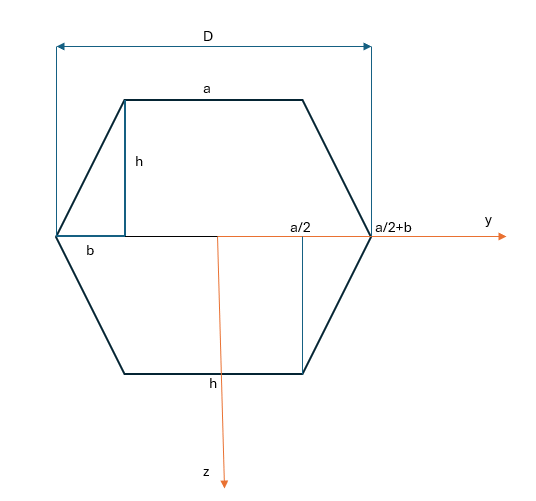
\includegraphics{idk.png}

Ze vztahů $D=a+2b$ a $\cos{60\degree}=\frac{b}{a}=\frac{1}{2}$ odvodíme $a=\frac{D}{2}$ a $b=\frac{a}{2}$.

Ze vztahů $\sin{60\degree}=\frac{h}{a}=\frac{\sqrt{3}}{2}$ odvodíme $h=\frac{\sqrt{3}}{2}a$.

Pro centrální kvadratické momenty platí:

\[ J_y=\iint\limits_{S} z^2\mathrm{d}S \] 
\[ J_z=\iint\limits_{S} y^2\mathrm{d}S \] 

Díky symetrii vždy stačí spočítat jen jeden kvadrant a výsledek vynásobit 4. Budeme počítat nejdřív $J_y$, přičemž rozdělíme obsah na dva: obdélník $S_1$ a trojúhelník $S_2$.

\[ J_y=\iint\limits_{S} z^2\mathrm{d}S = \iint\limits_{S_1} z^2\mathrm{d}S + \iint\limits_{S_2} z^2\mathrm{d}S\] 

Spočítáme nejdřív první integrál.

\[ \iint\limits_{S_1} z^2\mathrm{d}S = \int_{0}^{\frac{a}{2}}\mathrm{d}y \int_{0}^{h} z^2 \mathrm{d}z = \left[y\right]_0^{\frac{a}{2}} \left[\frac{z^3}{3}\right]_0^{\frac{\sqrt{3}}{2}a} 
= \frac{a}{2} \frac{\frac{3^{\frac{3}{2}}}{8}a^3}{3} = \frac{3^{\frac{3}{2}}}{48}a^4\] 

Ke spočítání druhého integrálu je dobré si uvědomit, že podle Steinerových vět posuvu, má na kvadratický moment vliv jen posun kolmý k ose momentu, tzn. že můžeme zjednodušit meze v integrálu:

\[ \iint\limits_{S_2} z^2\mathrm{d}S = \int_{0}^{h}\mathrm \int_{\frac{a}{2}}^{\frac{a}{2}+b} z^2 \mathrm {d}y{d}z = \int_{0}^{h}\mathrm \int_{0}^{b} z^2 \mathrm {d}y{d}z\] 

Dále potřebujeme odvodit funkci, která by vyjadřovala sklon trojúhelníku:

\[ z(0)=h=\frac{\sqrt{3}}{2}a \] 
\[ z(b)=0 \]

Řešením této soustavy dostáváme
\[ z(y)=-\frac{\sqrt{3}}{2}\frac{a}{b}+\frac{\sqrt{3}}{2}a \]

Nyní jen dosadíme do integrálu:

\[ \iint\limits_{S_2} z^2\mathrm{d}S = \int_{0}^{h} \int_{0}^{b} \left(-\frac{\sqrt{3}}{2}\frac{a}{b}y+\frac{\sqrt{3}}{2}a\right)^2 \mathrm{d}y \mathrm{d}z 
= \int_{0}^{\frac{\sqrt{3}}{2}a} \int_{0}^{b} \left(\frac{3a^2}{4b^2}y^2 - \frac{3a^2}{2b}y + \frac{3a^2}{4}\right) \mathrm{d}y \mathrm{d}z \]
\[= \frac{\sqrt{3}}{2}a \left[ \frac{3a^2}{4b^2} \frac{y^3}{3} - \frac{3a^2}{2b} \frac{y^2}{2} + \frac{3a^2}{4} y \right]_{0}^{b}
= \frac{\sqrt{3}}{2}a \left( \frac{3a^2 b^3}{12b^2} - \frac{3a^2 b^2}{4b} + \frac{3a^2 b}{4} \right)\]  
\[= \frac{\sqrt{3}}{2}a \left( \frac{3a^2 b}{12} - \frac{3a^2 b}{4} + \frac{3a^2 b}{4} \right)
=  = \frac{\sqrt{3}}{2}a \left( \frac{3a^3}{24} \right) = \frac{\sqrt{3}}{48} a^4\]

Pro kvadratický momement $J_y$ tedy platí

\[ J_y= 4 \left( \frac{3^{\frac{3}{2}}}{48} + \frac{\sqrt{3}}{48} \right) a^4 = \frac{3+\sqrt{3}}{12} \left( \frac{D}{2}\right)^4 = 3,608 D^4 \cdot10^{-2}\]

Nyní budeme počítat kvadratický moment $J_z$. K němu opět potřebujeme odvodit funkci $y(z)$.

\[ y(0)=\frac{a}{2}+b = a\] 
\[ y(h)=y\left(\frac{\sqrt{3}}{2}a\right)=\frac{a}{2}\]

Řešením této soustavy dostáváme
\[ y(z)=-\frac{1}{\sqrt{3}}z+a \]

Nyní dosadíme do integrálu:
\[ J_z=4\iint\limits_{S} y^2\mathrm{d}S = 4\int_{0}^{a}\mathrm{d}y \int_{0}^{\frac{\sqrt{3}}{2}a} \left(-\frac{1}{\sqrt{3}}z+a\right)^2\mathrm{d}z 
= 4\int_{0}^{a}\mathrm{d}y \int_{0}^{\frac{\sqrt{3}}{2}a} \left(\frac{1}{3}z^2-\frac{2}{\sqrt{3}}za+a^2\right)\mathrm{d}z\]
\[= 4\left[ y\right]_0^{a} \left[ \frac{1}{9}z^3-\frac{1}{\sqrt{3}}z^2a+za^2\right]_0^{\frac{\sqrt{3}}{2}a} = 4\left(\frac{\sqrt{3}}{24} -\frac{\sqrt{3}}{4}+ \frac{\sqrt{3}}{2}\right)a^4
= \frac{7\sqrt{3}}{6} \left(\frac{D}{2}\right)^4= 1,263 D^4 \cdot 10^{-1}\]



\end{document}
